\documentclass[11pt,a4paper]{article}
\usepackage[margin=2cm]{geometry}
\usepackage[T1]{fontenc}
\usepackage{mathptmx}
\usepackage{amsmath,amssymb}
\usepackage{graphicx}
\usepackage{xcolor}
\usepackage{enumitem}
\usepackage{array}
\usepackage{float}
\usepackage{colortbl}
\usepackage{needspace}
\usepackage[labelformat=empty,skip=4pt]{caption}
\usepackage[hidelinks]{hyperref}
\graphicspath{{figs/}}
\definecolor{navy}{HTML}{1B3755}
\definecolor{headc}{HTML}{E6ECF5}
\definecolor{okc}{HTML}{DFF3DF}
\definecolor{noc}{HTML}{FBE0E0}
\setlength{\parindent}{0pt}
\setlength{\parskip}{5pt}
\renewcommand{\arraystretch}{1.25}
\newcommand{\sect}[1]{\needspace{8\baselineskip}\bigskip{\Large\color{navy}\bfseries #1}\par\smallskip{\color{navy}\hrule height 0.8pt}\smallskip}
\newcommand{\sub}[1]{\needspace{5\baselineskip}\medskip{\large\color{navy}\bfseries #1}\par}
\newcommand{\say}[1]{\par\smallskip\noindent\fbox{\parbox{\dimexpr\linewidth-2\fboxsep-2\fboxrule}{\textbf{In one sentence:} #1}}\par}
\newcommand{\q}[2]{\par\needspace{4\baselineskip}\medskip\noindent\textbf{Q#1.\ #2}\par\noindent}
\newcommand{\hd}{\rowcolor{headc}}

\begin{document}
\begin{center}
{\LARGE\bfseries\color{navy} The EMT Simulation of the Study}\\[4pt]
{\large What it is, how it was done, what it shows, and how to defend it}\\[2pt]
IEEE 13-node feeder, DIgSILENT PowerFactory --- Jhala Nath Kafle (081MSPSE009)
\end{center}

\say{The EMT run is a movie of one fault: it shows the real current wave during two fast reclosing shots and
proves that fuse F671-2 survives the fast shots without DG (45\,\% of its melting heat) but melts during the
second shot with DG (100\,\% at 0.752\,s), because the DG raises the fuse current and keeps feeding the
fault while the recloser is open.}

\sect{1. What EMT is, in plain words}
The rest of the study uses \textbf{short-circuit calculations}. They give one number per fault: the RMS current
in steady state. That is a \emph{photograph}. An \textbf{electromagnetic-transient (EMT) simulation} solves the
network equations step by step in time (here every 0.1\,ms) and gives the \emph{instantaneous} current
wave, including what happens when breakers open and close. That is a \emph{movie}.

\begin{table}[H]\centering\small
\begin{tabular}{|p{3.6cm}|p{5.7cm}|p{5.7cm}|}\hline
\hd \textbf{Question} & \textbf{Short-circuit (RMS) study} & \textbf{EMT simulation} \\ \hline
What is calculated & one RMS current per fault & the current wave, point by point in time \\ \hline
Time & none: the fault is ``frozen'' & 0 to 2\,s in steps of 0.1\,ms \\ \hline
DC offset, first peak & not shown & shown \\ \hline
Generator & one fixed reactance & the machine's flux and rotor move: the current decays and the rotor
can lose step \\ \hline
Breaker opening and reclosing & not possible & scripted as switching events \\ \hline
Used in the study for & all 39 cells, all settings, the classification & one fault, to check the reclosing
\emph{sequence} \\ \hline
Cost & seconds for hundreds of faults & one fault per run, three runs per case \\ \hline
\end{tabular}
\end{table}

\textbf{Why the study needs it.} The classification asks one question per fault: \emph{does the fuse start to
melt before the recloser's fast trip?} It cannot say what happens over a whole reclosing sequence: trip,
dead time, reclose, trip again. The fuse does not forget the first shot when the second one comes. Only a
time-domain run can add the heating of successive shots and show what the DG does while the recloser is open.

\sect{2. The case that was simulated}
\begin{table}[H]\centering\small
\begin{tabular}{|p{5.2cm}|p{10.2cm}|}\hline
\hd \textbf{Item} & \textbf{Value and reason} \\ \hline
Fault & line-to-line, phases a--c, at node 684, through 0.2\,$\Omega$ --- the case of the reference method's
time-domain figure; node 684 only has phases a and c \\ \hline
Fault instant & 0.30\,s; the fault is permanent \\ \hline
Simulation & PowerFactory EMT (instantaneous values), step 0.1\,ms, 0 to 2.0\,s \\ \hline
Two runs & DG out of service, and DG in service (4.05\,MVA synchronous machine at 692) \\ \hline
Settings & conventional (single-setting) R2: fast plug 300\,A, TMS 0.1; delayed plug 600\,A, TMS 1.0 \\ \hline
Fuse watched & F671-2, A055C 300E, at the head of the lateral 671--684 \\ \hline
Reclosing sequence & two fast shots, dead time 0.2\,s (read from the reference figure), then the delayed
curve \\ \hline
Breaker time & 3 cycles = 0.050\,s added to every recloser trip \\ \hline
Measured & current into node 632 (the plotted wave), through R2, and through the fuse; phases a and c \\ \hline
\end{tabular}
\end{table}

\textbf{Where the devices are.} The fault at 684 is \emph{downstream} of R2. The fuse F671-2 is between node 671
and the fault. The DG at 692 is connected next to node 671, so it is \emph{between R2 and the fuse}. This position
is the whole story (Figure~1).

\begin{figure}[H]\centering
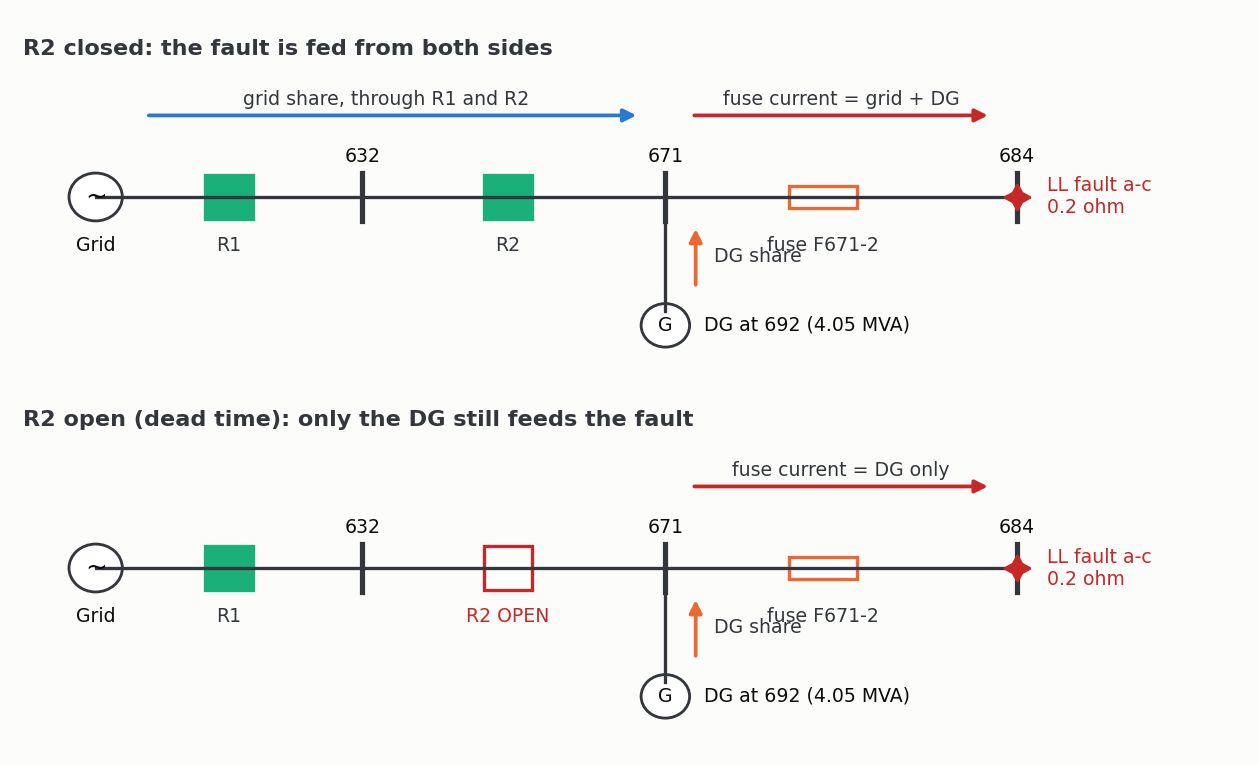
\includegraphics[width=0.86\textwidth]{emt_paths.png}
\caption*{\small Figure 1. Who feeds the fault. With R2 open the grid is cut off, but the DG is still connected
to the fault through the fuse.}
\end{figure}

\sect{3. How the simulation was run}
PowerFactory's own relay and fuse elements were switched out of service for the EMT runs. Instead, every
switching time was calculated from the \emph{same curves used in the rest of the study}, applied to the simulated
current. This keeps the sequence transparent: every time in the result can be traced to a curve and a current.
It takes three passes per case.

\begin{table}[H]\centering\small
\begin{tabular}{|c|p{5.3cm}|p{8.6cm}|}\hline
\hd \textbf{Pass} & \textbf{What is simulated} & \textbf{What is taken from it} \\ \hline
1 & the fault only, no switching & the one-cycle RMS current through R2 $\rightarrow$ R2's fast time from its
curve, plus the breaker time \\ \hline
2 & fault + two fast trips and two recloses & the RMS current through the fuse at every time step $\rightarrow$
fuse heating; when it melts and when it clears; R2's delayed timer after the last reclose \\ \hline
3 & the whole sequence, with the fuse opening & the final wave that is plotted in the report \\ \hline
\end{tabular}
\end{table}

\sub{3.1 From the wave to an RMS value}
A relay curve and a fuse curve are given in RMS amperes, but the EMT gives instantaneous values. So the wave is
converted with a \textbf{one-cycle moving RMS}: at every instant, the RMS of the last 1/60\,s. The larger of
phases a and c is used.

\sub{3.2 The recloser}
\[
t_{\text{trip}} = t_{R2,\text{fast}}(I_{R2}) + 3\ \text{cycles}
\]
Without DG: $I_{R2}=2607$\,A $\rightarrow$ curve time 0.070\,s $+$ 0.050\,s $=$ 0.120\,s, so R2 opens at
$0.30+0.120=0.420$\,s. With DG: $I_{R2}=2436$\,A $\rightarrow$ 0.076\,s $+$ 0.050\,s $=$ 0.126\,s, R2 opens
at 0.426\,s. R2 recloses 0.2\,s later and the same fast time runs again.

\sub{3.3 The fuse: heat accumulation}
A fuse melts when its element has absorbed enough heat. At a constant current $I$ that takes the
minimum-melting time $t_{MMT}(I)$ of its curve. When the current changes or is interrupted, each small time
step $\Delta t$ uses up a fraction $\Delta t/t_{MMT}(I)$ of the melting heat:
\[
H(t)=\sum \frac{\Delta t}{t_{MMT}\big(I_{fuse}(t)\big)}, \qquad \text{the fuse melts when } H = 1\ (100\,\%).
\]
The same sum with the total-clearing time $t_{TCT}$ gives the instant at which the fuse has cleared.
\textbf{No cooling is assumed} while the recloser is open, which is on the safe side and reasonable for a dead
time of 0.2\,s.

\sect{4. Reading the current wave}
\begin{figure}[H]\centering
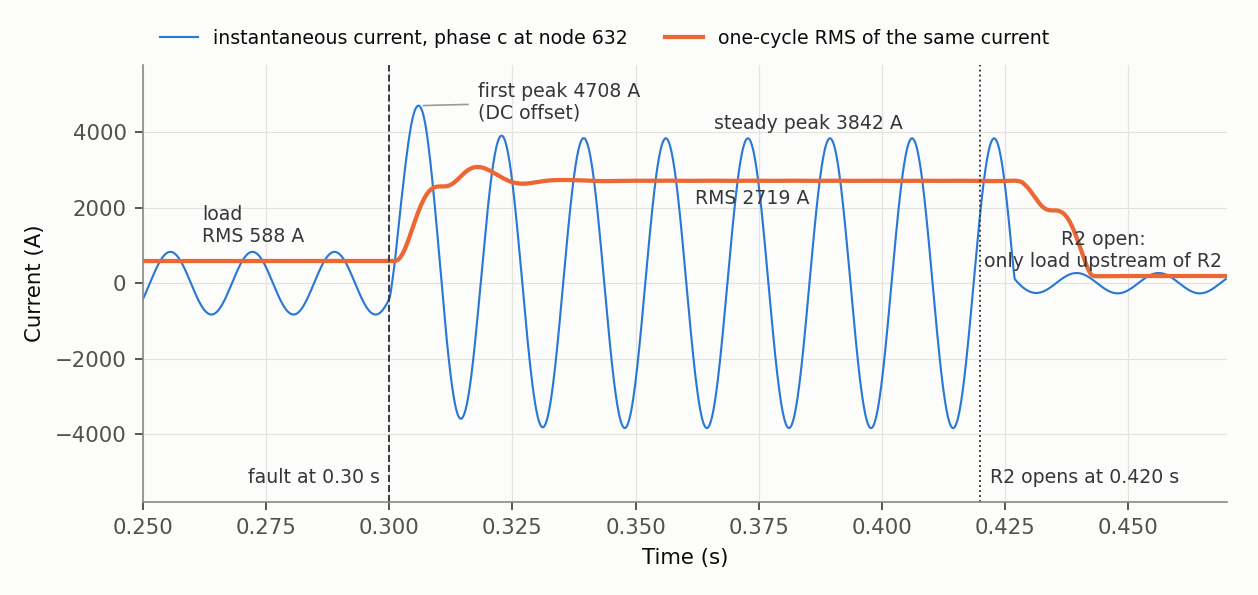
\includegraphics[width=0.9\textwidth]{emt_anatomy.png}
\caption*{\small Figure 2. The first fast shot without DG, phase c of the current into node 632.}
\end{figure}

\begin{itemize}[leftmargin=*,itemsep=2pt]
\item \textbf{Before 0.30\,s:} load current, 588\,A RMS.
\item \textbf{First peak 4708\,A:} higher than the later peaks. This is the \textbf{DC offset}: the current in
an inductive circuit cannot jump, so a decaying DC component is added to the AC wave. Its size depends on the
instant of the fault on the voltage wave and on the X/R ratio; it is gone after about one cycle here.
\item \textbf{Steady peak 3842\,A, RMS 2719\,A:} the ratio is $3842/2719 = 1.413 = \sqrt{2}$, as it must be for a
sine wave. A short-circuit calculation only gives this RMS value.
\item \textbf{0.420\,s:} R2 opens. The current does not fall to zero at node 632, because the loads between
the substation and R2 are still supplied (about 190\,A).
\item \textbf{The RMS line} needs one cycle to rise and one to fall: that is the one-cycle window.
\end{itemize}

\begin{table}[H]\centering\small
\begin{tabular}{|l|c|c|c|c|}\hline
\hd & \multicolumn{2}{c|}{\textbf{Without DG}} & \multicolumn{2}{c|}{\textbf{With DG}} \\ \hline
\hd \textbf{Current into node 632 (A)} & \textbf{phase a} & \textbf{phase c} & \textbf{phase a} & \textbf{phase c} \\ \hline
Before the fault, RMS & 557 & 588 & 261 & 286 \\ \hline
During the fault, RMS & 2362 & 2719 & 2443 & 2353 \\ \hline
First peak & 4288 & 4708 & 3805 & 3653 \\ \hline
Steady peak & 3338 & 3842 & 3517 & 3414 \\ \hline
While R2 is open, RMS & 97 & 191 & 91 & 185 \\ \hline
\end{tabular}
\end{table}
With the DG the pre-fault current from the grid is about half (261 against 557\,A): the DG supplies part of the
load locally.

\sect{5. The result: the two sequences}
\begin{figure}[H]\centering
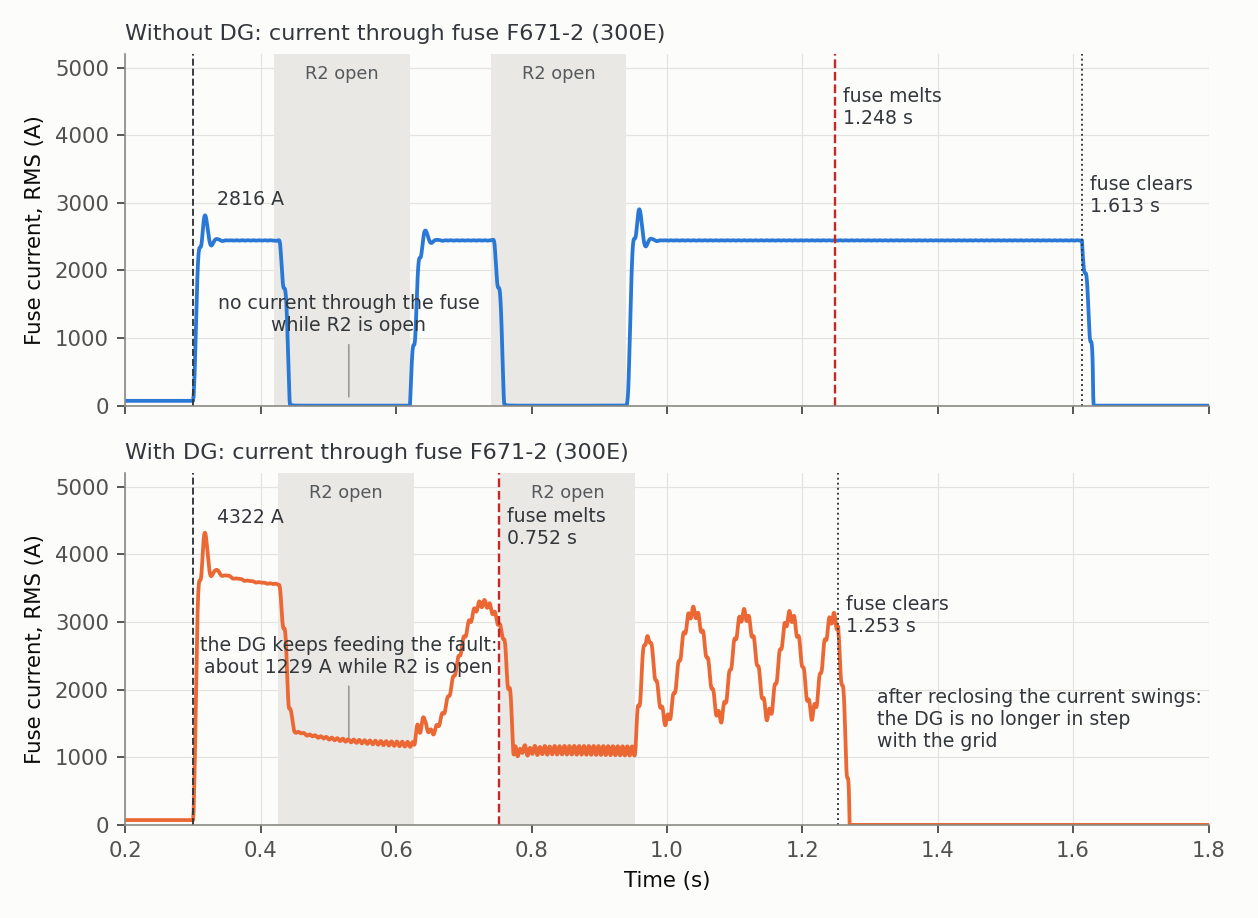
\includegraphics[width=0.92\textwidth]{emt_sequence.png}
\caption*{\small Figure 3. RMS current through fuse F671-2 over the whole sequence. Grey: R2 is open.}
\end{figure}

\begin{table}[H]\centering\small
\begin{tabular}{|p{6.2cm}|c|c|p{4.6cm}|}\hline
\hd \textbf{Event (time in s)} & \textbf{Without DG} & \textbf{With DG} & \textbf{Comment} \\ \hline
Fault initiated & 0.300 & 0.300 & \\ \hline
R2 fast trip 1 & 0.420 & 0.426 & R2 sees less current with DG \\ \hline
R2 reclose 1 & 0.620 & 0.626 & dead time 0.2\,s \\ \hline
\rowcolor{noc} Fuse F671-2 melts (with DG) & --- & 0.752 & during fast shot 2 \\ \hline
R2 fast trip 2 & 0.740 & 0.753 & \\ \hline
R2 reclose 2 & 0.940 & 0.953 & now on the delayed curve \\ \hline
\rowcolor{okc} Fuse F671-2 melts (without DG) & 1.248 & --- & after both fast shots \\ \hline
Fuse F671-2 has cleared & 1.613 & 1.253 & \\ \hline
\hd Fuse heat when the fast shots are over & 45\,\% & 105\,\% & of the melting heat \\ \hline
\end{tabular}
\end{table}

\begin{figure}[H]\centering
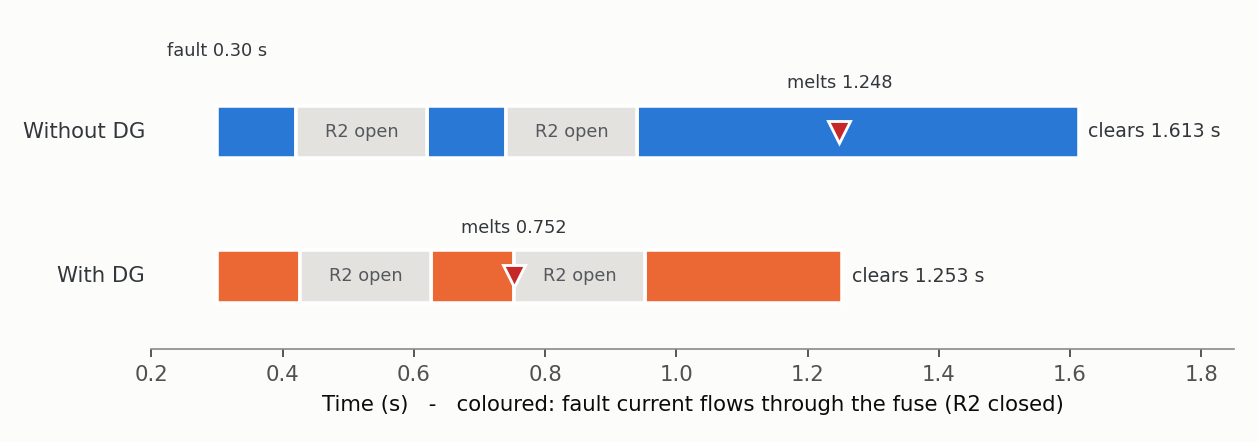
\includegraphics[width=0.88\textwidth]{emt_timeline.png}
\caption*{\small Figure 4. The two sequences on one time axis.}
\end{figure}

\textbf{Without DG --- fuse saving works.} The fuse reaches only 45\,\% of its melting heat during the two fast
shots. If the fault had been temporary, it would have been cleared by one of the two fast trips and the fuse
would still be intact. Because the fault is permanent, it is still there after the second reclose; R2 is now on
its delayed curve (2.67\,s at this current), so the fuse has time to melt (1.248\,s) and clear (1.613\,s)
\emph{before} R2 would trip again. Only the lateral 671--684 is lost. This is exactly the intended sequence.

\textbf{With DG --- fuse saving is lost.} The fuse melts at 0.752\,s, one millisecond before the second fast
trip. A temporary fault would now cost a fuse and a permanent outage of the lateral, which is what the fast
shots were supposed to prevent.

\sect{6. Why the fuse melts with DG: the heat budget}
\begin{figure}[H]\centering
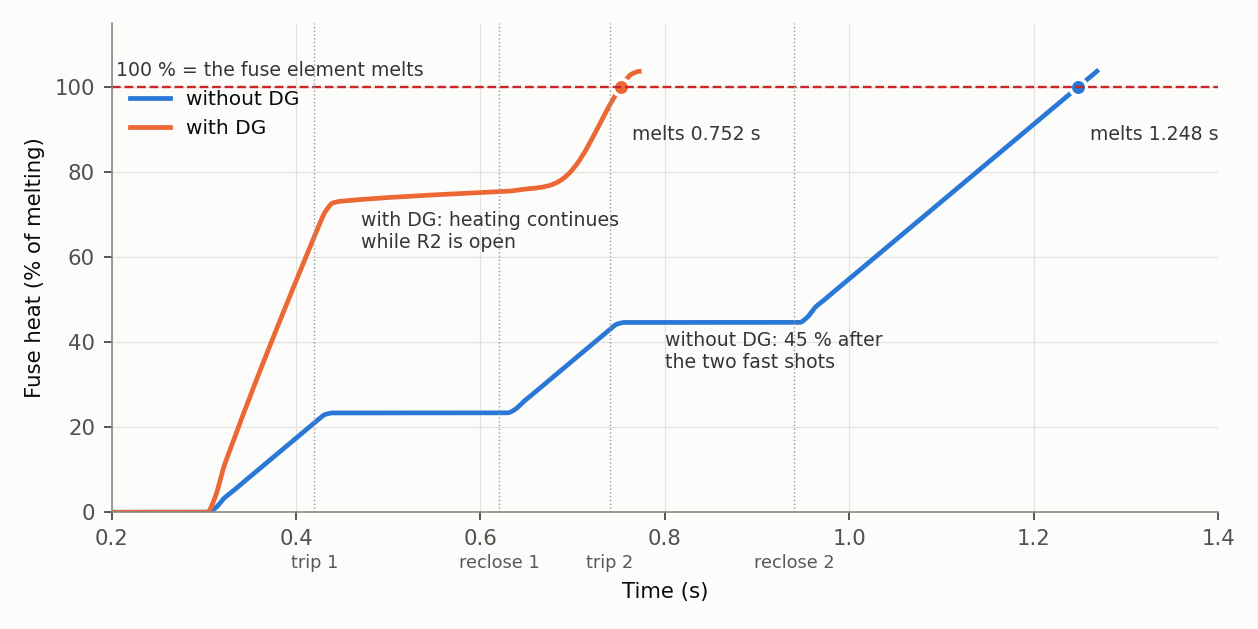
\includegraphics[width=0.9\textwidth]{emt_heat.png}
\caption*{\small Figure 5. Accumulated fuse heat $H(t)$. Flat parts: no heating. The orange line keeps rising
between trip 1 and reclose 1, because the DG still feeds the fault.}
\end{figure}

\begin{table}[H]\centering\small
\begin{tabular}{|p{4.9cm}|c|c|c|c|}\hline
\hd & \multicolumn{2}{c|}{\textbf{Without DG}} & \multicolumn{2}{c|}{\textbf{With DG}} \\ \hline
\hd \textbf{Interval} & \textbf{heat added} & \textbf{total} & \textbf{heat added} & \textbf{total} \\ \hline
Fast shot 1 (fault to trip 1) & 21\,\% & 21\,\% & 68\,\% & 68\,\% \\ \hline
Dead time 1 (R2 open) & 2\,\% & 23\,\% & 7\,\% & 75\,\% \\ \hline
Fast shot 2 (reclose 1 to trip 2) & 20\,\% & 43\,\% & 25\,\% & \cellcolor{noc}100\,\% \\ \hline
Dead time 2 (R2 open) & 2\,\% & \cellcolor{okc}45\,\% & 5\,\% & 105\,\% \\ \hline
\end{tabular}
\end{table}
{\small The small amounts in the dead time without DG are the last cycle of fault current before the breaker
contacts part (the RMS window is one cycle long).}

Three things act together, all caused by the DG:
\begin{enumerate}[leftmargin=*,itemsep=2pt]
\item \textbf{The fuse carries more current.} 4322\,A at the start against 2816\,A without DG (grid + DG).
At 4322\,A the fuse melts in 0.120\,s; at 2816\,A in 0.361\,s. One shot now costs 68\,\% instead of 21\,\%.
\item \textbf{The recloser sees less and is slower.} R2 carries only the grid share: 2436\,A against 2607\,A, so
its fast shot lasts 0.126\,s instead of 0.120\,s.
\item \textbf{The DG keeps feeding the fault while R2 is open.} About 1230\,A flows through the fuse during the
dead time, adding 7\,\% and then 5\,\%. Without DG the dead time is a real pause.
\end{enumerate}

\sub{A hand check you can do on the board}
Without DG the fuse carries a steady 2441\,A. Its curve gives $t_{MMT}(2441\,\text{A}) = 0.553$\,s. The fuse
actually carried fault current for
\[
0.120\ (\text{shot 1}) + 0.120\ (\text{shot 2}) + (1.248-0.940)\ (\text{after reclose 2}) = 0.548\ \text{s}
\]
before it melted. The 5\,ms difference is the higher current of the first cycle of each shot (DC offset). So
the simulated melting instant agrees with the fuse curve.

\sect{7. What the EMT showed that the curves alone could not}
\begin{enumerate}[leftmargin=*,itemsep=3pt]
\item \textbf{Heating adds up over the shots.} The classification compares one fast trip with the melting
time. For this fault with DG it would say the fuse survives one shot (68\,\%). The EMT shows that two shots plus
the dead-time infeed do not fit into the fuse.
\item \textbf{The DG current decays.} The fuse current falls from 4322\,A to about 3570\,A within the first shot:
a synchronous machine starts on its subtransient reactance and its contribution then falls towards the
transient value. A short-circuit calculation gives only the initial value.
\item \textbf{The DG feeds the fault during the dead time.} This is invisible in any calculation that looks at
one network state at a time. It also means the arc of a \emph{temporary} fault may not extinguish while R2 is
open --- the purpose of the dead time is defeated.
\item \textbf{The DG falls out of step.} After each reclose the current through the fuse is no longer steady: it
swings with a period of about 0.07\,s (a difference of about 14\,Hz between the DG and the grid). During the
fault and the dead time the machine cannot deliver its power, so its rotor speeds up (its mechanical starting
time is only 1.5\,s), and R2 recloses onto a machine that is no longer synchronised.
\item \textbf{The margin matters.} At the initial 4322\,A the fuse curve gives 0.120\,s, and R2 with its breaker
needs 0.126\,s. With the zero-margin rule (curve time 0.076\,s) the first shot looks safe; with the three-cycle
breaker time it is at the edge. This is the same effect that reduces the held cells from 38 to 31 in the margin
study.
\end{enumerate}

\sect{8. How it fits the conclusions of the report}
\begin{itemize}[leftmargin=*,itemsep=2pt]
\item It is a \textbf{time-domain confirmation} of the main cause of the problem: the fuse carries the grid and
the DG current, the recloser only the grid share.
\item It shows the \textbf{limit} stated in the report: for faults \emph{downstream} of R2 the DG feeds the
fault directly. The dual setting cannot help there, because R2's forward group is the same in both schemes and
no setting of R2 changes what the DG delivers. That is why the EMT was run with the conventional settings.
\item It supports the \textbf{future work} listed in the report: disconnection of the DG during the reclosing
dead time, and a practical margin.
\end{itemize}

\sect{9. Limitations --- say these yourself before you are asked}
\begin{itemize}[leftmargin=*,itemsep=2pt]
\item \textbf{One fault only.} One location, one fault type, one fault impedance, conventional settings. It is
a check of the sequence, not a second classification.
\item \textbf{The protection is scripted.} Trip and melt instants come from the device curves applied to the
simulated RMS current, in three passes; the relay and fuse elements of PowerFactory do not act in the EMT run.
(They were checked separately: 1896 operating times within 1.22\,\%.)
\item \textbf{The fuse is a heat sum,} without cooling and without an arc model. The clearing instant is the
$t_{TCT}$ sum, not a simulated arc.
\item \textbf{The dead time (0.2\,s) and the breaker time (3 cycles) are assumed;} the dead time was read from
the reference figure.
\item \textbf{The DG stays connected.} No anti-islanding or under/over-frequency protection is modelled. In
practice the DG protection would be expected to trip it during the dead time, which would remove the dead-time
infeed and the out-of-step reclosing --- but not the higher fuse current of the first shot.
\item \textbf{Step 0.1\,ms} is right for the 60\,Hz current and its DC offset; the run was not made to study
switching overvoltages or travelling waves.
\item \textbf{No DSDR case in EMT,} for the reason given in Section 8.
\end{itemize}

\newpage
\sect{10. Questions you may be asked}

\sub{Basics}
\q{1}{What is an EMT simulation?}
A simulation that solves the network's differential equations step by step in time and gives the
instantaneous voltages and currents. Here: step 0.1\,ms, 2\,s, in PowerFactory.

\q{2}{How is it different from your short-circuit study?}
The short-circuit study gives one RMS value for a frozen network. The EMT gives the wave: DC offset, decay of
the generator current, and the effect of opening and reclosing. I used the short-circuit study for all 39 cells
and the EMT for one fault, to check the sequence in time.

\q{3}{Why did you need it at all? The classification already tells you whether coordination holds.}
The classification checks one fast trip against the fuse melting time. A reclosing sequence has two fast shots
and dead times, and the fuse heating adds up. Only a time-domain run shows that, and shows what the DG does
while the recloser is open.

\q{4}{Why this fault: LL a--c at 684 through 0.2\,$\Omega$?}
It is the fault of the reference method's time-domain figure, so the sequence can be set against it. Node 684
has only phases a and c, so an a--c fault is the largest phase fault there.

\q{5}{Why a step of 0.1\,ms?}
One 60\,Hz cycle is 16.7\,ms, so there are 167 points per cycle: more than enough for the fundamental current
and its DC offset, which is all the relay and fuse curves need. I did not study switching overvoltages, which
would need a smaller step and frequency-dependent line models.

\sub{The modelling}
\q{6}{How is the recloser modelled?}
As a three-phase switch on line 632--671 with scripted events. The trip instant is R2's fast-curve time at the
simulated RMS current plus three cycles of breaker time; it recloses after a dead time of 0.2\,s; two fast
shots; after the second reclose the delayed curve applies.

\q{7}{Why did you switch off PowerFactory's own relay and fuse models?}
To keep one consistent set of curves for the whole study and to make every instant traceable to a curve and a
current. If both the scripted events and the built-in models acted, the sequence would be ambiguous. The
built-in models were checked separately and agree within 1.22\,\%.

\q{8}{How do you get an RMS value out of an instantaneous wave?}
A one-cycle moving RMS: at each instant the RMS of the previous 1/60\,s. I take the larger of phases a and c.

\q{9}{How is the fuse modelled?}
As accumulated heat: every time step adds $\Delta t/t_{MMT}(I)$. The fuse melts when the sum reaches 1. The same
sum with $t_{TCT}$ gives the clearing instant. It is the usual way to apply a time--current curve to a current
that is not constant.

\q{10}{A fuse cools down during the dead time. Did you include that?}
No. Cooling is neglected, which is on the safe side: it overestimates the heat slightly. With a dead time of
0.2\,s the cooling of the element is small. Including it would not change the conclusion: with DG the fuse is
at 68\,\% after one shot and the DG keeps heating it during the dead time.

\q{11}{Where do the 0.2\,s dead time and the two fast shots come from?}
From the reference figure: its reclosing instants are 0.2\,s after the trips, and it shows two fast operations.
Two fast and then delayed operations is also the usual fuse-saving sequence.

\sub{The results}
\q{12}{Explain the 45\,\%.}
Without DG the fuse carries about 2441\,A, where it needs 0.553\,s to melt. Each fast shot lasts 0.120\,s, so
each uses $0.120/0.553\approx 21$--$22\,\%$. Two shots: about 45\,\%. The fuse is intact after the fast shots.

\q{13}{Why does the fuse melt with the DG?}
Three reasons. The fuse carries grid plus DG current, 4322\,A instead of 2816\,A, so it heats about three times
faster. R2 carries only the grid share, 2436\,A instead of 2607\,A, so it trips slightly later. And the DG
keeps about 1230\,A flowing through the fuse while R2 is open. Total after two shots: 105\,\%.

\q{14}{The first peak is 4708\,A but the later peaks are 3842\,A. Why?}
DC offset. The current cannot jump in an inductive circuit, so a decaying DC component appears; it depends on
the fault instant on the voltage wave and on X/R. It is gone after about a cycle. The steady peak over the RMS
is exactly $\sqrt{2}$.

\q{15}{With the DG the fuse current falls during the first shot. Why?}
That is the synchronous machine: its fault contribution starts at the subtransient level and decays towards the
transient level. A short-circuit calculation only gives the initial value; the EMT shows the decay.

\q{16}{After reclosing with the DG, the current swings up and down. What is that?}
The DG has lost synchronism. During the fault and the dead time it cannot deliver its power, so the rotor
accelerates; the machine is small, with a mechanical starting time of 1.5\,s. When R2 recloses, the grid and
the DG are no longer in step and the current beats with a period of about 0.07\,s. It is a known risk of
reclosing onto a feeder with a rotating DG.

\q{17}{When R2 opens, the current at node 632 does not go to zero. Why?}
The plotted current is the feeder current arriving at node 632. The loads and laterals between the substation
and R2 are still supplied: about 97 and 191\,A in the two phases.

\q{18}{Without DG the fuse still blows at 1.248\,s. Is that not a failure?}
No, it is the intended behaviour. The fault is permanent. The fast shots give a temporary fault two chances
to clear without losing the fuse. When the fault is still there, R2 goes to its delayed curve, 2.67\,s at this
current, and the fuse clears at 1.613\,s before R2 trips again. Only the faulted lateral is lost.

\q{19}{How do you know the EMT result is right?}
Three checks. The steady peak over RMS is $\sqrt{2}$. The pre-fault current is the load current of the load
flow. And the hand check: the fuse carried fault current for $0.120+0.120+0.308=0.548$\,s before melting,
against $t_{MMT}=0.553$\,s at 2441\,A from its curve.

\sub{Tricky ones}
\q{20}{Your classification is about the DSDR. Why is the EMT run with conventional settings?}
The fault at 684 is downstream of R2. There R2 carries forward current in both schemes, and its forward group
is the same, so the sequence would be identical. The EMT was made to verify the reclosing sequence and the
effect of the DG, following the reference figure. An EMT run of an upstream fault with the reverse group is
future work.

\q{21}{So does the DSDR solve the problem shown by the EMT?}
No, and the report says so. For faults downstream of R2 the DG feeds the fault directly through the fuse and
no setting of R2 changes that. The DSDR restores coordination for faults \emph{between the grid and the DG}.
That is why the report calls the DSDR necessary but not sufficient.

\q{22}{The static classification and the EMT: do they agree?}
They answer different questions and they are consistent. With the zero-margin rule the fuse survives the
first fast trip with DG, and the EMT also shows 68\,\% after one shot. The EMT adds the second shot and the
dead-time infeed, which bring it to 100\,\%.

\q{23}{In a real network the DG would be tripped by its own protection. Then your result is not realistic?}
The DG protection is not modelled, and I state that as a limitation. If the DG tripped during the first dead
time, the dead-time infeed and the out-of-step reclosing would disappear. But the first shot would still cost
68\,\% instead of 21\,\%, because that happens before any DG protection can act. So the main finding stays: the
DG uses up most of the fuse's margin.

\q{24}{What would you do to save the fuse in this case?}
A larger or slower fuse on the lateral, checked again for selectivity with the fuses below it; a faster fast
curve is not available, because R2 is already at its lowest dial; and disconnecting the DG before the first
reclose. These are the fuse revision and the future work of the report.

\q{25}{Is the DG current during the dead time dangerous in itself?}
Yes for fuse saving: a temporary fault is an arc, and the arc needs the current to stop in order to
extinguish. If the DG keeps about 1.2\,kA flowing, the arc may not go out, and the reclose finds the fault
still there.

\q{26}{Is one EMT case enough?}
For its purpose, yes: it verifies the sequence and shows the mechanism in time. It is not a replacement for
the classification, which covers all 39 cells. More EMT cases --- other locations, the reverse group, DG
protection --- are a natural extension.

\sect{11. Numbers to remember}
\begin{table}[H]\centering\small
\begin{tabular}{|p{7.2cm}|c|c|}\hline
\hd \textbf{Quantity} & \textbf{Without DG} & \textbf{With DG} \\ \hline
Current through R2 (RMS) & 2607\,A & 2436\,A \\ \hline
R2 fast shot, curve + breaker & 0.070 + 0.050 = 0.120\,s & 0.076 + 0.050 = 0.126\,s \\ \hline
Fuse current at the start of the fault (RMS) & 2816\,A & 4322\,A \\ \hline
Fuse melting time at that current & 0.361\,s & 0.120\,s \\ \hline
Fuse current while R2 is open & 0 & about 1230\,A \\ \hline
Fuse heat after the two fast shots & 45\,\% & 105\,\% \\ \hline
Fuse melts & 1.248\,s & 0.752\,s \\ \hline
Fuse has cleared & 1.613\,s & 1.253\,s \\ \hline
Fuse saving & \cellcolor{okc}works & \cellcolor{noc}lost \\ \hline
\end{tabular}
\end{table}
Fault at 0.30\,s; dead time 0.2\,s; breaker 3 cycles; step 0.1\,ms; fuse F671-2 300E; R2 fast plug 300\,A,
TMS 0.1.

\end{document}
